\begin{wrapfigure}{r}{70mm}
\centering
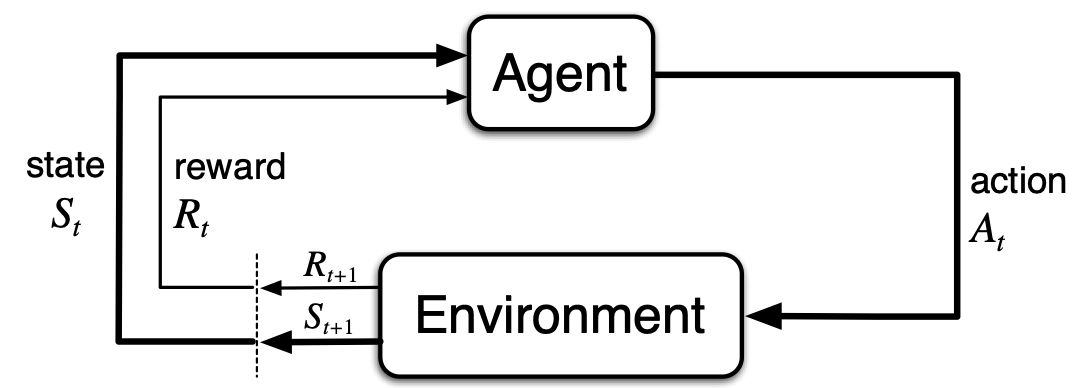
\includegraphics[width=0.5\textwidth]{Figures/agent_environment_model.png}
\caption{Schematic illustration of Reinforcement Learning, copied from
\cite{sutton_reinforcement_2018}}
\label{fig:agent_environment_model}
\end{wrapfigure}
Reinforcement Learning is a branch of Machine Learning that aims to train an
agent in a dynamic environment. At each time step $t$, the agent takes an
action $A_t$ based on the observed environment state $S_t$. The
environment reacts by providing a reward signal $R_{t+1} \in \mathbb{R}$. The
goal of the agent is to select its actions in such a way that the sum of
reward signals (called return) is maximized. The action selection strategy is
referred to as policy. A schematic illustration of an interaction
between agent and environment is shown in Figure~\ref{fig:agent_environment_model}.
In our experiments, the action is the choice of speed for
each pump given a state represented by sensor readings,
and the reward is determined by the energy efficiency and satisfactory operating conditions
(see Section~\ref{sec:experimental_setup}).

The Soft Actor-Critic algorithm (SAC)
\cite{haarnoja_soft_2018} has
particularly promising properties for the pump scheduling task: It was
designed to handle large and continuous action spaces, which makes it a good
candidate for the simultaneous control of multiple variable-speed pumps. SAC
employs a replay buffer, meaning that it stores previous experience to be
re-used in training, which improves data efficiency. A specialty of SAC is the training objective: In
addition to the common RL goal of finding the policy that will maximize the
expected return, a separate term for the maximization
of entropy in the probabilistic policy is introduced.
% \begin{equation}
% J(\pi) = \sum_{t=1}^T \mathbb{E}_{(s_t, a_t) \sim \rho(\pi)} \left[ r(s_t, a_t) +
% \alpha \mathcal{H}(\pi(\cdot | s_t))\right]
% \label{eq:sac_objective}
% \end{equation}
% In Equation ~\ref{eq:sac_objective}, $J$ is the full objective, $\pi$ is the
% policy, $t$ denotes a timestep, and $s$ and $a$ are state and action,
% respectively. The distribution $\rho$ describes the probability of taking
% action $a$ in state $s$ under the current policy. Entropy is denoted by
% $\mathcal{H}$ and $\alpha$ is a weighting factor.
This leads to better exploration behaviour of the agent and more robust
training over all. For a detailed description of SAC, we refer the
interested reader to the original paper \cite{haarnoja_soft_2018} as well as
to the following online resource for an
overview\footnote{\href{https://spinningup.openai.com/en/latest/algorithms/sac.html}{https://spinningup.openai.com/en/latest/algorithms/sac.html}}.
